
%%%%%%%%%%%%%%%%%%%%%%%%%%%%%%%%%%%%%%%%%%%%%%%%%%%%%%%%%%%%%%%%%%%%%%%%%%%%%%%
%             Hardware support
%%%%%%%%%%%%%%%%%%%%%%%%%%%%%%%%%%%%%%%%%%%%%%%%%%%%%%%%%%%%%%%%%%%%%%%%%%%%%%%
\section{WR Hardware Support}
\label{sec:hwSupport}

SyncE is responsible for clock syntonization in the WRN. In the SyncE scheme, the 
reference clock (125MHz) is used to encode the outgoing data
stream. The same clock is retrieved on the other side of the physical
link using the \textit{Clock Recovery System} (CRS, section~\ref{sec:wrCRS}). 
Having the same frequency allows us to use phase detector technologies as a means of evaluating
delays. WR implements Digital Dual Mixer Time Difference (DDMTD) \cite{biblio:WRproject}
phase detection. The measurement of phase is used for 
increasing the precision of timestamps beyond the resolution allowed by the 125MHz clock.
This process \modified{is} described in the next section. 
The DDMTD phase detection is also used to obtain 
\textit{the transmit/receive (Tx/Rx) latencies} (section~\ref{sec:TxRxLatencies})
\modified{and compare frequencies in the CRS}.

%%%%%%%%%%%%%%%%%%%%%%%%%%%%%%%%%%%%%%%%%%%%%%%%%%%%%%%%%%%%%%%%%%%%%%%%%%%%%%%
%             timestamps and fine delay
%%%%%%%%%%%%%%%%%%%%%%%%%%%%%%%%%%%%%%%%%%%%%%%%%%%%%%%%%%%%%%%%%%%%%%%%%%%%%%%


\subsection{Fine Delay Measurement}
\label{sec:fineDelay}
We call \textit{Fine Delay Measurement} the process during which the DDMTD-detected round-trip phase
shift ($phase_{MM}$ in \figurename~\ref{fig:wrLink}) is used to enhance 
timestamp precision and to calculate the precise round-trip delay 
($delay_{MM}$). 
During the fine delay process only the reception timestamp ($t_2$, $t_4$) 
measurements need to be improved as they are transmitted and timestamped in
different clock domains.

A basic timestamp (to be enhanced) is obtained by the detection of 
the Start-of-Frame Delimiter (SFD) in the Physical Coding Sublayer (PCS).
In order to acquire a precision-improved timestamp, we need to eliminate the possible 
$\pm$~1~LSB error \modified{(8ns)} %Pablo's remark to add unit
due to jitter of clock signals and clock-domain crossing. 
Therefore, the Time-Stamping Unit (TSU) produces timestamps on both the rising 
and falling edges of the clock, and later in the process one of them is chosen.
The process involves three steps (see \cite{biblio:TomekMSc} for details):
% \begin{figure}[!t]
% \centering
% \includegraphics[width=2.5in]{fig/preciseTimestamp.ps}
% \caption{Timestamp enhancing \cite{biblio:TomekMSc}.}
% \label{fig:preciseTimestamp}
% \end{figure}
% % Only the reception timestamps ($t_2$, $t_4$)
% need to be enhanced as they are transmitted and timestamped in
% different clock domains. 
%(see \figurename~\ref{fig:preciseTimestamp} for $t_{4}$ to $t_{p4}$
%enhancement explanation)
\begin{enumerate}
   \item rising/falling edge timestamp choice ($t_f$ or $t_r$),
   \item calculating the picosecond part, checking
         its sign and adding a clock period if necessary,
   \item extending timestamps with the picosecond part ($t_{2p}$, $t_{4p}$).
 \end{enumerate}
The modified timestamps are used to calculate the precise round-trip delay
(\figurename~\ref{fig:wrLink}):
\begin{equation}
  \label{eq:delaymm}
  delay_{MM} = (t_{4p}-t_{1}) - (t_{3}-t_{2p})
\end{equation}



%%%%%%%%%%%%%%%%%%%%%%%%%%%%%%%%%%%%%%%%%%%%%%%%%%%%%%%%%%%%%%%%%%%%%%%%%%%%%%%
%             WR Clock Recovery System
%%%%%%%%%%%%%%%%%%%%%%%%%%%%%%%%%%%%%%%%%%%%%%%%%%%%%%%%%%%%%%%%%%%%%%%%%%%%%%%

\subsection{\modified{Robust} Clock Recovery System}
\label{sec:wrCRS}

\begin{figure}[!t]
\centering
%\includegraphics[width=2.95in]{fig/wrCRS.eps}
\includegraphics[height=0.95in]{robustness/wrCRS.eps}
\caption{\modified{White Rabbit Clock Recovery System.}}
\label{fig:PLL}
\end{figure}

The White Rabbit implementation of the CRS (WR CRS) is explained in
detail in \cite{biblio:TomekMSc}, \figurename~\ref{fig:PLL} presents
a very simplified overview of the WR CRS. It is designed to accommodate
multiple sources of frequency (physical links) with a single source
being used (active) at a given time. A seamless switching of the
active source is one of the goals of the design to enable network
topology redundancy \modified{and, as a consequence, offer robust and stable synchronization 
(see section~\ref{sec:wrBMC})}.


All input reference clocks (\textit{ref clk}) and a feedback clock (\textit{feedback clk}) are
fed into DDMTD and degliching units (\textit{DDMTD}). The input clocks are mixed by the DDMTDs with 
the offset frequency (\ref{equation:offsetFreq}) which is derived from the 
active ref~clock. The frequency-mixing results in a low frequency clock signal which maintains the
original 
phase shift. 
\begin{equation}
  \label{equation:offsetFreq}
     f_{offset}[ns] =  125[MHz] * \frac{2^N}{2^N+ \Delta}% \mbox{ , }N=14 \mbox{ \& } \Delta=1
\end{equation}
A prototype implementation using $N=14$ and $\Delta=1$ has demonstrated satisfactory performance 
\cite{biblio:TomekMSc}. Each output of the DDMTD reference channel is compared with the output
of the feedback channel in the \textit{phase and frequency error detection} units. The additional 
input to the units is the \textit{WRPTP phase shift} obtained in the \textit{Fine Delay
Measurement}. The phase and frequency error (\textit{phase and freq error}) between the feedback
clock and each reference clock, corrected by WRPTP phase shift, is calculated and fed into the
multiplexer (\textit{MUX}).
During normal operation, the active reference clock (from the Primary Slave port, 
section~\ref{sec:wrBMC}) is used to feed the PI controller and produce the output reference signal.
However, if the malfunction of the active ref clock is detected, the switch-over process
takes place: the MUX is switched to feed the PI with the error data from another reference channel
(from the Secondary Slave port).
\modified{An estimate of the average phase and frequency errors can be provided to the PI controller
to improve hold-over performance if all the reference channels fail.}



The active clock malfunction takes 3 consecutive invalid symbols
($\sim24ns$) to detect while the phase and frequency error detection is performed
at a low frequency (kHz). Therefore, the continuity of the synchronization is 
guaranteed during the switch-over. 



%%%%%%%%%%%%%%%%%%%%%%%%%%%%%%%%%%%%%%%%%%%%%%%%%%%%%%%%%%%%%%%%%%%%%%%%%%%%%%%
%             Tx/Rx calibration
%%%%%%%%%%%%%%%%%%%%%%%%%%%%%%%%%%%%%%%%%%%%%%%%%%%%%%%%%%%%%%%%%%%%%%%%%%%%%%%

\subsection{The transmit/receive (Tx/Rx) latencies} 
\label{sec:TxRxLatencies}

\begin{figure}[!t]
\centering
%\includegraphics[width=1.74in]{fig/calibration.eps}
\includegraphics[height=0.95in]{misc/calibration.eps}
\caption{\modified{Rx/Tx latency measurement \cite{biblio:WRPTP}. }}
\label{fig:calibration}
\end{figure}

The transmit/receive (Tx/Rx) latencies in most PHYs vary for
each \modified{Phase-Locked Loop/Clock Data Recovery (PLL/CDR)} 
%\modified{PLL/CDR\footnote{\modified{Phase-Locked Loop/Clock Data Recovery}}} 
lock cycle, but stay constant once the PHY is
locked. This is the case of the PHY used in the WR Switch prototype
(TCK1221), therefore an Tx/Rx latency measurement is required. Tx
latency is measured by feeding the transmit path with a sequence of
RD+ K28.7 code-group (Appendix~36A.2 of \cite{biblio:IEEE8023}). 
Such signal creates a 125MHz clock on
the SerDes I/O. Since the Tx clock frequency is also 125MHz, the DDMTD
can be used to measure the phase shift between the SerDes I/O and the
Tx clock, effectively measuring Tx latency. By receiving the K28.7
signal from the link partner, the Rx latency can be measured using the
same method. This process, depicted in \figurename~\ref{fig:calibration},
is performed during the WR Link Setup (section~\ref{sec:wrLinkSetup}).


